

% Gradient Info
  
\tikzset {_ec7nzqwik/.code = {\pgfsetadditionalshadetransform{ \pgftransformshift{\pgfpoint{0 bp } { 0 bp }  }  \pgftransformrotate{-265 }  \pgftransformscale{2 }  }}}
\pgfdeclarehorizontalshading{_xyfuj5rm5}{150bp}{rgb(0bp)=(1,1,1);
rgb(37.5bp)=(1,1,1);
rgb(62.5bp)=(0.29,0.56,0.89);
rgb(100bp)=(0.29,0.56,0.89)}

% Gradient Info
  
\tikzset {_rjiyvzeb0/.code = {\pgfsetadditionalshadetransform{ \pgftransformshift{\pgfpoint{0 bp } { 0 bp }  }  \pgftransformrotate{-73 }  \pgftransformscale{2 }  }}}
\pgfdeclarehorizontalshading{_f7g2os25i}{150bp}{rgb(0bp)=(1,1,1);
rgb(37.5bp)=(1,1,1);
rgb(62.5bp)=(0.29,0.56,0.89);
rgb(100bp)=(0.29,0.56,0.89)}
\tikzset{every picture/.style={line width=0.75pt}} %set default line width to 0.75pt        

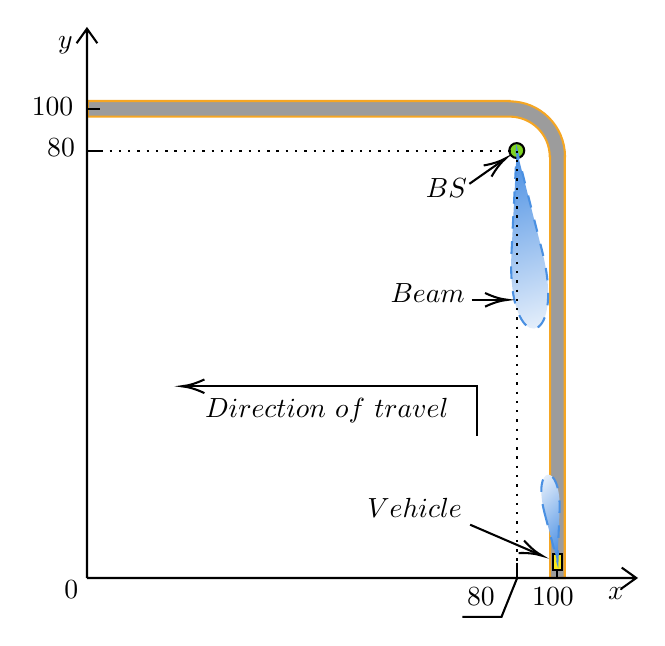
\begin{tikzpicture}[x=0.75pt,y=0.75pt,yscale=-1,xscale=1]
%uncomment if require: \path (0,389); %set diagram left start at 0, and has height of 389

%Shape: Path Data [id:dp9439264762383368] 
\draw  [color={rgb, 255:red, 245; green, 166; blue, 35 }  ,draw opacity=1 ][fill={rgb, 255:red, 156; green, 156; blue, 156 }  ,fill opacity=1 ] (425.26,116.06) -- (425.11,116.06) -- (425.11,319.23) -- (418.05,319.23) -- (418.05,116.12) -- (417.9,116.12) .. controls (417.81,105.52) and (409.19,96.94) .. (398.56,96.94) -- (398.56,96.98) -- (195.32,96.98) -- (195.32,89.43) -- (398.56,89.43) -- (398.56,89.58) .. controls (413.23,89.58) and (425.14,101.42) .. (425.26,116.06) -- cycle ;
%Shape: Axis 2D [id:dp06192362645207816] 
\draw  (194.94,319.23) -- (459.58,319.23)(194.94,54.59) -- (194.94,319.23) -- cycle (452.58,314.23) -- (459.58,319.23) -- (452.58,324.23) (189.94,61.59) -- (194.94,54.59) -- (199.94,61.59)  ;
%Shape: Ellipse [id:dp6223646892502144] 
\draw  [fill={rgb, 255:red, 126; green, 211; blue, 33 }  ,fill opacity=1 ] (398.42,113.29) .. controls (398.42,111.31) and (400.03,109.71) .. (402.01,109.71) .. controls (403.99,109.71) and (405.6,111.31) .. (405.6,113.29) .. controls (405.6,115.27) and (403.99,116.88) .. (402.01,116.88) .. controls (400.03,116.88) and (398.42,115.27) .. (398.42,113.29) -- cycle ;
%Straight Lines [id:da38619721366461013] 
\draw    (379.17,129.34) -- (395.28,118.03) ;
\draw [shift={(396.91,116.88)}, rotate = 504.93] [color={rgb, 255:red, 0; green, 0; blue, 0 }  ][line width=0.75]    (10.93,-3.29) .. controls (6.95,-1.4) and (3.31,-0.3) .. (0,0) .. controls (3.31,0.3) and (6.95,1.4) .. (10.93,3.29)   ;
%Straight Lines [id:da15022537128136448] 
\draw    (379.55,293.56) -- (412.44,307.74) ;
\draw [shift={(414.28,308.53)}, rotate = 203.32] [color={rgb, 255:red, 0; green, 0; blue, 0 }  ][line width=0.75]    (10.93,-3.29) .. controls (6.95,-1.4) and (3.31,-0.3) .. (0,0) .. controls (3.31,0.3) and (6.95,1.4) .. (10.93,3.29)   ;
%Straight Lines [id:da7854826192671283] 
\draw    (382.82,250.64) -- (382.82,226.86) -- (242.58,226.86) ;
\draw [shift={(240.58,226.86)}, rotate = 360] [color={rgb, 255:red, 0; green, 0; blue, 0 }  ][line width=0.75]    (10.93,-3.29) .. controls (6.95,-1.4) and (3.31,-0.3) .. (0,0) .. controls (3.31,0.3) and (6.95,1.4) .. (10.93,3.29)   ;
%Shape: Regular Polygon [id:dp9427611315548852] 
\path  [shading=_xyfuj5rm5,_ec7nzqwik] (399.45,162.89) .. controls (401.94,112.62) and (402.01,113.29) .. (402.01,113.29) .. controls (402.01,113.29) and (402.01,113.29) .. (414.17,161.44) .. controls (426.34,209.59) and (396.95,213.15) .. (399.45,162.89) -- cycle ; % for fading 
 \draw  [color={rgb, 255:red, 74; green, 144; blue, 226 }  ,draw opacity=1 ][dash pattern={on 4.5pt off 4.5pt}][line width=0.75]  (399.45,162.89) .. controls (401.94,112.62) and (402.01,113.29) .. (402.01,113.29) .. controls (402.01,113.29) and (402.01,113.29) .. (414.17,161.44) .. controls (426.34,209.59) and (396.95,213.15) .. (399.45,162.89) -- cycle ; % for border 

%Straight Lines [id:da7817331508669928] 
\draw    (194.57,93.21) -- (201.36,93.21) ;
%Straight Lines [id:da8717772464646777] 
\draw    (194.57,113.29) -- (201.36,113.29) ;
%Straight Lines [id:da7724065322091858] 
\draw  [dash pattern={on 0.84pt off 2.51pt}]  (201.36,113.29) -- (402.01,113.29) ;
%Straight Lines [id:da16520179645725375] 
\draw    (402.2,311.86) -- (402.2,319.23) ;
%Straight Lines [id:da717938560212316] 
\draw  [dash pattern={on 0.84pt off 2.51pt}]  (402.01,113.29) -- (402.01,311.86) ;
%Straight Lines [id:da5108761534053126] 
\draw    (421.61,311.49) -- (421.61,318.85) ;
%Shape: Rectangle [id:dp2495833516134348] 
\draw  [color={rgb, 255:red, 0; green, 0; blue, 0 }  ,draw opacity=1 ][fill={rgb, 255:red, 248; green, 231; blue, 28 }  ,fill opacity=1 ] (419.56,307.52) -- (423.66,307.52) -- (423.66,315.45) -- (419.56,315.45) -- cycle ;
%Shape: Regular Polygon [id:dp8848176218099444] 
\path  [shading=_f7g2os25i,_rjiyvzeb0] (415.4,287.93) .. controls (421.65,311.82) and (421.61,311.49) .. (421.61,311.49) .. controls (421.61,311.49) and (421.61,311.49) .. (422.62,287.15) .. controls (423.62,262.8) and (409.15,264.04) .. (415.4,287.93) -- cycle ; % for fading 
 \draw  [color={rgb, 255:red, 74; green, 144; blue, 226 }  ,draw opacity=1 ][dash pattern={on 4.5pt off 4.5pt}][line width=0.75]  (415.4,287.93) .. controls (421.65,311.82) and (421.61,311.49) .. (421.61,311.49) .. controls (421.61,311.49) and (421.61,311.49) .. (422.62,287.15) .. controls (423.62,262.8) and (409.15,264.04) .. (415.4,287.93) -- cycle ; % for border 

%Straight Lines [id:da471299456937862] 
\draw    (375.77,337.96) -- (394.65,337.96) -- (402.2,319.23) ;
%Straight Lines [id:da2760255541693942] 
\draw    (380.3,185.21) -- (395.67,185.21) ;
\draw [shift={(397.67,185.21)}, rotate = 180] [color={rgb, 255:red, 0; green, 0; blue, 0 }  ][line width=0.75]    (10.93,-3.29) .. controls (6.95,-1.4) and (3.31,-0.3) .. (0,0) .. controls (3.31,0.3) and (6.95,1.4) .. (10.93,3.29)   ;

% Text Node
\draw (444.52,322.54) node [anchor=north west][inner sep=0.75pt]    {$x$};
% Text Node
\draw (179.53,56.79) node [anchor=north west][inner sep=0.75pt]    {$y$};
% Text Node
\draw (182.53,318.79) node [anchor=north west][inner sep=0.75pt]    {$0$};
% Text Node
\draw (356.73,125.5) node [anchor=north west][inner sep=0.75pt]    {$BS$};
% Text Node
\draw (328.54,279.27) node [anchor=north west][inner sep=0.75pt]    {$Vehicle$};
% Text Node
\draw (166.87,86.24) node [anchor=north west][inner sep=0.75pt]    {$100$};
% Text Node
\draw (174.26,106.12) node [anchor=north west][inner sep=0.75pt]    {$80$};
% Text Node
\draw (407.95,322.16) node [anchor=north west][inner sep=0.75pt]    {$100$};
% Text Node
\draw (376.59,322.29) node [anchor=north west][inner sep=0.75pt]    {$80$};
% Text Node
\draw (250.33,231.08) node [anchor=north west][inner sep=0.75pt]    {$Direction\ of\ travel$};
% Text Node
\draw (339.69,176.09) node [anchor=north west][inner sep=0.75pt]    {$Beam$};


\end{tikzpicture}